\documentclass[12pt]{article}
\usepackage{mathpazo}
\usepackage{maybemath,xspace,setspace,fancybox,fancyvrb}
\usepackage{a4wide,url,relsize,underscore}
\usepackage[colorlinks=true,bookmarks=true]{hyperref}
\newcommand{\maybemath}{\texttt{maybemath}\xspace}
\newcommand{\hepthesis}{\texttt{hepthesis}\xspace}

\onehalfspacing
\DefineShortVerb{\|}
\setlength{\fboxsep}{10pt}
\addtolength{\fboxrule}{0.6\fboxrule}

\newcommand{\hepthesisversion}{v1.5.2}
\author{Andy Buckley, \texttt{andy@insectnation.org}}
\title{hepthesis \hepthesisversion \\ \smaller A class for typesetting academic theses}

%% Bold tt font
\DeclareFontShape{OT1}{cmtt}{bx}{n}{<5><6><7><8><9><10><10.95><12><14.4><17.28><20.74><24.88>cmttb10}{}

\newcommand{\Or}{\texorpdfstring{\ensuremath{\vert}\xspace}{or}}
\newcommand{\manifestsAs}{\texorpdfstring{\ensuremath{\Rightarrow\quad}\xspace}{->}}
\newcommand{\texcmd}[1]{\texorpdfstring{\texttt{\char`\\#1}}{#1}}
\newcommand{\texenv}[1]{\texorpdfstring{\texttt{#1}}{#1}}
\newcommand{\texopt}[1]{\texorpdfstring{\texttt{#1}}{#1}}
\newcommand{\texarg}[1]{\texorpdfstring{\texttt{\{#1\}}}{\textbraceleft#1\textbraceright}}
\newcommand{\texargoptgen}[1]{\texorpdfstring{\texttt{[}\gen{#1}\texttt{]}}{\textbraceleft<#1>\textbraceright}}
\newcommand{\texarggen}[1]{\texorpdfstring{\texttt{\{}\gen{#1}\texttt{\}}}{\textbraceleft<#1>\textbraceright}}
\newcommand{\gen}[1]{\ensuremath{\langle\text{\mdseries\itshape#1\/}\rangle}}
\newcommand{\texpkg}[1]{#1}
\newcommand{\texoption}[1]{\texopt{#1}}

\newenvironment{snippet}{\Verbatim}{\endVerbatim}
\newenvironment{fsnippet}%
  {\VerbatimEnvironment
    \begin{Sbox}\begin{minipage}{0.82\textwidth}\begin{Verbatim}}%
  {\end{Verbatim}\end{minipage}\end{Sbox}
    \setlength{\fboxsep}{12pt}\vspace*{4mm}\newline\fbox{\TheSbox}\vspace{4mm}\par\noindent}

% \newenvironment{snippet}%
% {\begin{minted}{latex}}{\end{minted}}
% \newenvironment{fsnippet}%
%   {\begin{Sbox}\begin{minipage}{0.82\textwidth}\begin{minted}{latex}}%
%   {\end{minted}\end{minipage}\end{Sbox}
%     \setlength{\fboxsep}{12pt}\vspace*{4mm}\newline\fbox{\TheSbox}\vspace{4mm}}

\begin{document}
{\larger[3] \sffamily \bfseries \maketitle}

\abstract{%
  The \hepthesis class provides an attractive framework in which to write a PhD
  or Masters' degree dissertation. The commands provided by this package permit
  most structural aspects of the thesis to be defined more or less semantically,
  rather than in terms of raw text sizings and position shifts.
}


\section{Introduction}
When I began my PhD in 2001, I was surprised to find that there was no standard
\LaTeX{} thesis class used by students in my field (\emph{h}igh-\emph{e}nergy
\emph{p}article physics, hence the ``hep''). In retrospect, this is not so
surprising --- research groups often have an informal system of handing down
slightly tailored thesis templates (complete with in line \texcmd{vspace}s,
\texcmd{Huge}s and all the rest) through generations of students without ever
formalising the style and attempting to do it ``properly''.

By the time it came to write my own thesis it was obvious that I would only
retain my sanity through measures of extreme procrastination and so this package
came to be. It has now been edited and hacked on and off since roughly mid-2004,
taking stylistic features from other theses that I've thought attractive and
adding features based on my own pickiness and user requests. The typography
isn't motivated by any formal understanding of the subject, though, so I'm sure
there's still plenty of room for improvement.

This document documents the structure of \hepthesis and how to make it work
with you rather than against you. I may be unable to resist including other
hints and tips on how to make your thesis-writing go smoothly. Please contact me
with suggested improvements, either to the package or to this documentation.


\section{Features}
Why would you want to use \hepthesis? Here's a list of features, so you can
decide for yourself:

\begin{itemize}
\item Semantic macros for defining the front page, abstract, preface, acknowledgements, etc.
\item Macros for quotes, including a full-page quote and chapter-wise quotes
\item Attractive header and footer structures
\item Pre-set margins suitable for binding or for screen viewing
\item Nicely (re-)defined figure, table and equation environments
\item Optional mode for generating hyper-links when building PDF files
\item Built-in draft copy mode with line numbering
\item Maths in section titles etc. will automatically be boldened if appropriate
\end{itemize}


\section{Recommended usage}
The basic usage mode for \hepthesis is to place
%
\begin{snippet}
\documentclass{hepthesis}
\end{snippet}
%
in the preamble of your document. This will then set up the document's appearance and
provide the \hepthesis macros as do the standard \LaTeX{} classes like |article|
and |report|. A more sophisticated and flexible approach is described in
Appendix~\ref{app:DerivedClass}.

Although strictly unrelated to \hepthesis, it is usual to write each thesis
chapter as a separate |.tex| file and to include it with
\texcmd{include} or \texcmd{input}. You may find it useful to set your
|LATEXINPUTS| environment variable to ensure that the \texcmd{input}'d
files are found by \LaTeX.

\hepthesis takes several optional arguments. Personally, I use
%
\begin{snippet}
\documentclass[hyperpdf,bindnopdf]{hepthesis}
\end{snippet}
%
which produces page-centered, hyper-linked PDF files and PostScript files with
margins suitable for binding and no hyper-links, depending on whether you build
the document using |latex| or |pdflatex|. The details of the \hepthesis options
are described in Section~\ref{sec:Options} of this document.


\section{Requirements}
As \hepthesis aims to allow produce a fairly final version of a thesis without
much additional tweaking, there are quite a few required packages. Most should
be natively available in your \TeX{} distribution; the rest from CTAN.

Here's the mandatory packages:
\begin{itemize}
\item \textbf{scrbook\,\cite{scrbook}} (from KOMA-scripts)
\item \textbf{setspace\,\cite{setspace}}
\item \textbf{fancyhdr\,\cite{fancyhdr}}
\item \textbf{rotating\,\cite{rotating}}
\item \textbf{comment\,\cite{comment}}
\item \textbf{tocbibind\,\cite{tocbibind}}
\item \textbf{caption\,\cite{caption}}
\item \textbf{changepage\,\cite{changepage}}
\item \textbf{varwidth\,\cite{varwidth}}
\end{itemize}

\vspace{0.4cm}
\noindent\fbox{\begin{minipage}{0.85\textwidth}\textsl{
%
Note that the \texpkg{subfig}\,\cite{subfig} (previously \texpkg{subfigure})
and \texpkg{ccaption}\,\cite{ccaption} packages, which were required up to
version 1.3, are no longer needed.
If you need sub-figures then you should \texcmd{usepackage} the package as
usual in your document preamble or custom class file, and make use of the
\texcmd{ContinuedFloat} command for continuation captions, which is
provided by the mandatory \texpkg{caption} package.
%
}\end{minipage}}
\vspace{0.4cm}

Additionally, there are several packages which are only required depending on
the class options:

\begin{itemize}
%\item \textbf{cite\,\cite{cite}}
\item \textbf{csquotes\,\cite{csquotes}:} very standard. Quotation commands will use this if loaded.
\item \textbf{babel\,\cite{babel}:} very standard. Quotation commands will use this if loaded.
\item \textbf{a4wide\,\cite{a4wide}:} very standard. Disabled with any paper size option other than |a4paper|
\item \textbf{amsmath\,\cite{amsmath}:} very, \emph{very} standard. Disabled with the |noams| option
\item \textbf{hyperref\,\cite{hyperref}:} very standard. Enabled with the |hyper| option
\item \textbf{booktabs\,\cite{booktabs}:} very standard. Disable with the |nobooktabs| option
\item \textbf{draftcopy\,\cite{draftcopy}:} very standard. Enable with the |draft| option
\item \textbf{lineno\,\cite{lineno}:} non-standard (?). Enable with the |draft| option
\item \textbf{titling\,\cite{titling}:} non-standard (?). Enable with the |titling| option
\end{itemize}

Some other handy packages (which aren't required at all for compatibility with
|hepthesis| but may well help you to write your thesis) are summarised in
Section~\ref{sec:ExtraPackages}.

\subsection{Troublesome interactions}
Unfortunately not all \LaTeX{} packages get on well with each other --- if
you are unlucky then you may get some of \TeX's wondertully cryptic error
messages on trying to use \texpkg{hepthesis}. Here are the problems that I'm
aware of\dots

\begin{itemize}
\item
If you have problems with \LaTeX{} complaining about bad definitions of
\texcmd{pdfstringdefPreHook}, you may be using an old version of \texpkg{csquotes},
which doesn't interface well to \texpkg{hyperref}. I think this is fixed in
\texpkg{csquotes} version 3.2 and later --- it certainly works for version
3.7. Try including the \texpkg{csquotes} package with
%
\begin{snippet}
\usepackage{csquotes}[2007/03/25]
\end{snippet}
%
so that sufficiently recent version will be used.

\item
Similarly, version 0.9 of the \texpkg{varwidth} package has a deformed version
string which means that the package doesn't load properly. This version seems to
have made its way into some \LaTeX{} package distributions, so if you see such
an error then version 0.9a or later can be obtained from CTAN and will work
properly. \texpkg{hepthesis} will check to make sure that the version is as
required and issue a warning if the version on your system is earlier than those
known to be good.

\end{itemize}


\section{Class options}
\label{sec:Options}

\subsection{\texopt{oneside} \Or \texopt{twoside}}
Typeset the thesis for printing in one- or two-sided format: for example, you
may wish to present preview and draft copies in two-sided format, but the final
submission may be required to be single-sided. Changing to single-sided form
will remove the blank facing pages and only use the margins and header/footer
format specified for right-hand pages.

\subsection{\texopt{bind} \Or \texopt{nobind} \Or \texopt{bindnopdf}}
Set the margins to be suitable for printing or screen-viewing. Using the
\texopt{bind} option produces larger inner margins, so that left- and
right-facing pages have LR-reflection symmetry. Using the \texopt{nobind}
option makes the margins equal, so that the pages don't jump around when you
flick through them in |gv| or Adobe Acrobat. The \texopt{bindnopdf} option
will use binding margins when making a PostScript document and screen-view
margins when building a PDF. Note that this option requires some carefulness
with the |.aux| files: this is described in Appendix \ref{app:AuxFileProblem}.

\subsection{\texopt{ams} \Or \texopt{noams}}
Make use of the AMS mathematical package. This re-defines several \hepthesis
mathematical environments using more powerful macros and is enabled by default.
If you don't plan on having any maths in your thesis, then disabling this option
may speed up your build-time a little.

\subsection{\texopt{alphafoot}}
Use alphanumeric footnote markers.

\subsection{\texopt{hidefront} \Or \texopt{hideback} \Or \texopt{hidefrontback}}
Useful for draft builds, these options respectively hide the front matter, the
back matter or both from the \LaTeX{} compilation, giving a faster build time
and meaning you don't have to flick through 20 pages of garbage before
proof-checking the first real content. Note that hiding the back matter will
fail to include the bit where you generate your bibliography, so unless you make
a work-around, all your citations will break.

\subsection{\texopt{draft}}
Prints ``DRAFT'' diagonally across the pages and numbers the lines, suitable for
proof-reading. This makes use of the standard |draftcopy| and the less-standard
|lineno| packages.

\subsection{\texopt{sftitles}}
Uses a sans-serif font for the title page and all chapter, section and
subsection headings.

\subsection{\texopt{rmtitles}}
Uses a serif (roman) font for the title page and all chapter, section and
subsection headings (this is the default).

\subsection{\texopt{booktabs} \Or \texopt{nobooktabs}}
Use the |booktabs| package to define the \hepthesis tabular environment.
|booktabs| produces publication quality tables, as opposed to \TeX's rather
ropey defaults, and so this option is enabled by default. You can disable it if
your thesis doesn't have any tables and get a slightly faster build, but it is
strongly encouraged that any table presentation uses the |booktabs| look and
feel because it's so much better!

\subsection{\texopt{hyper}}
The |hyper| option is used to activate the |hyperref| package, with some reasonably
sensible default options. Essentially, it's equivalent to putting
%
\begin{snippet}
\usepackage[colorlinks=true,pdfpagemode=FullScreen, \
            bookmarks=true]{hyperref}
\end{snippet}
%
in the preamble of your document.

\subsection{\texopt{hyperpdf}}
|hyperpdf| has the effect of the |hyper| option when building PDF output, and no
effect at all if building PostScript. This can be handy if you consider the PDFs
to be for screen-reading purposes and the PS for printing: you probably don't
want to print a version where all the references and URLs are coloured! Note
that this option requires some carefulness with the |.aux| file, since
alternating between PS and PDF builds involves repeatedly writing and removing
hyperref tokens. A solution to this is described in Appendix \ref{app:AuxFileProblem}.

\subsection{\texopt{index}}
Include the |makeidx| package, to allow an index to be built. Note that you have
to do this by hand and that it's probably best done as a retrospective feature
after you've written the thesis. Not many people want to spend \emph{more} time
with their thesis when they've done enough to pass!

\subsection{\texopt{titling}}
Use the |titling| package to redefine the \texcmd{title} and \texcmd{author}
commands so that their arguments are available through the document as
\texcmd{thetitle} and \texcmd{theauthor}. This is used, for example, by the
\texcmd{titlepage} command. If this option isn't passed, a more basic attempt is
made to do this definition without needing an external package.  It's unclear
whether titling really helps but there may be complicated cases (such as those
where the author includes a \texcmd{thanks}) where |titling| may do a better
job. This is untested, though, and the result of using \texcmd{thanks} in a
|hepthesis| document is to be considered undefined.

\subsection{\texopt{a4paper} \Or \texopt{a4narrow} \Or \texopt{letterpaper} \Or \dots}
Choose the paper size. Duh.


\section{Environments and commands}
The \hepthesis environments and commands are a mix of new macros and tweaked
versions of existing standard ones. The ones that re-define standard macros
can't be disabled (at least, not in this version), so if you don't like them
then you can either hack \hepthesis to be the way you'd like (preferably in a
nice way which I can integrate into a future release) or use something else. The
choice is yours!

Here are the environments and commands, roughly in the order that you'd use them:

\subsection{\texcmd{set{\dots}spacing}\texarggen{spacing}}
A selection of spacing commands are available to change the overall line spacing
of the thesis, or to change the spacing within specific document sections if for
some reason you want to do that. (Personally, I wouldn't --- inconsistent spacing
is very disconcerting.) Here are the available commands, explicitly:
\begin{itemize}
\item \texcmd{setspacing} --- set the following spacings all at once;
\item \texcmd{setfrontmatterspacing}
\item \texcmd{setmainmatterspacing}
\item \texcmd{setappendixspacing}
\item \texcmd{setbackmatterspacing}
\end{itemize}
%
Each command takes a single argument, which can take the values |single|,
|onehalf| and |double|, for single spacing, one-and-a-half spacing
and double spacing respectively. The default is |onehalf|, since I think
that looks most elegant. If making a draft version, double spacing might be
useful since it leaves a bit of room for annotations. I can't recommend single
spacing --- it just looks cramped.
%
\begin{fsnippet}
\documentclass[...]{hepthesis}
\setmainmatterspacing{double}
...
\begin{document}
  ...
\end{fsnippet}


\subsection{\texcmd{set{\dots}extramargins}\texarggen{length}}
A selection of commands are available to change the text width on a per-section
basis. These shouldn't be tweaked too much, but in case you need it, the ability
for configuration is available. The text width itself is not explicitly
specified --- instead the commands take as an argument the width to be added to
both margins. Unless explicitly specified below, all these lengths are zero by
default so any use of these commands with a positive argument is likely to
reduce the text width. Here are the ``large-scale'' extra margins commands:
%
\begin{itemize}
\item \texcmd{setextramargins}\texarggen{len} --- set the following lengths all at once;
\item \texcmd{setfrontmatterextramargins}\texarggen{len}
\item \texcmd{setmainmatterextramargins}\texarggen{len}
\item \texcmd{setappendixextramargins}\texarggen{len}
\item \texcmd{setbackmatterextramargins}\texarggen{len}
\end{itemize}
%
The following commands all add extra margin widths to subsections within the
front matter. Note that they apply \emph{in addition} to the front matter length.
%
\begin{itemize}
\item \texcmd{setabstractextramargins}\texarggen{len} --- |1.5cm| by default;
\item \texcmd{setdeclarationextramargins}\texarggen{len} --- |1.5cm| by default;
\item \texcmd{setacknowledgementsextramargins}\texarggen{len}
\item \texcmd{setprefaceextramargins}\texarggen{len}
\end{itemize}
%
Each command takes a single argument, which is just a \TeX{} length. Here's an example:
\nobreak
%
\begin{fsnippet}
\documentclass[...]{hepthesis}
\setfrontmatterextramargins{1.5}
...
\begin{document}
  ...
\end{fsnippet}


%% TODO Change in v1.5
\subsection{\texcmd{title}\texarggen{title} and \texcmd{author}\texarggen{author}}
The usual commands for setting the author and title. Don't use \texcmd{thanks} in
the \hepthesis author argument: the results are undefined!
%
\begin{fsnippet}
\title{A study of \BToKPi decays with the \LHCb experiment}
\author{Andrew Gordon Buckley}
...
\begin{document}
  ...
\end{fsnippet}

Once these commands have been executed, the title and author strings are available
via the \texcmd{thetitle} and \texcmd{theauthor} commands. These are used by
\texcmd{titlepage}.

N.B. Up to version 1.3, a special \texcmd{definethesis} command was used to specify
the thesis author and title. While this is still retained for backwards compatibility,
it is deprecated and you should use the standard \texcmd{title} and \texcmd{author}
macros instead. \textbf{\texcmd{definethesis} will be removed in version 1.5}


\subsection{\texenv{frontmatter}, \texenv{mainmatter}, \texenv{appendices} and \texenv{backmatter} environments}
Use these to delimit the auxiliary parts of your thesis from the main feature
(being all that clever work you spent years working on). In practice, these
commands change the page-numbering style and set/reset some section counters
appropriately: the frontmatter and backmatter environments will not use chapter
numbering but will insert the un-numbered chapter titles in the table of
contents. Note that this means appendices should be placed in the appendices
environment between mainmatter and backmatter, rather than in the back matter
itself, which is intended for such things as the bibliography, colophon etc.

\subsection{\texcmd{titlepage}}
The \texcmd{titlepage} macro generates a title page for the thesis and as such
should probably be the first item in the front matter. It takes two arguments:
an optional elaboration of the author name and the description of the award for
which the thesis is being submitted. You may need to use a different macro if
your institution has a very different prescribed format for the layout of thesis
title pages: in such a case, the \texcmd{theauthor} and \texcmd{thetitle}
commands will probably be useful. Here's an example of usage:
%
\begin{fsnippet}
\titlepage[of \\ Churchill College]%
{A dissertation submitted to the University of Cambridge\\
for the degree of Doctor of Philosophy}
\end{fsnippet}
%
Additionally, the \texcmd{maketitle} command has been redefined to behave as
\texcmd{titlepage} with two empty arguments. This is only provided to not
confuse users who convert to |hepthesis| from a standard \LaTeX{} class and
expect \texcmd{maketitle} to work: \texcmd{titlepage} is a more powerful
command and should be used by those who are aware of it. That includes you!

\subsection{\texenv{abstract} environment}
Where you present the summary of your thesis: this should be within the
\texenv{frontmatter} environment. The \texenv{abstract} environment takes one
optional argument, which will be the heading above the abstract. If this isn't
specified, the heading will simply be ``Abstract''. This may be useful for
providing a stand-alone summary page, with a snippet like:
%
\begin{fsnippet}
\begin{abstract}%
  [\smaller\thetitle\\ \vspace*{1cm} \smaller{\theauthor}]
\thispagestyle{empty}
This thesis describes all the really cool work I did on...
\end{abstract}
\end{fsnippet}

\subsection{\texenv{declaration} environment}
Where you declare that the thesis was all your own work, lies within word
limits, etc. Use it in the front matter area, of course, with something like
%
\begin{fsnippet}
\begin{declaration}
  This dissertation is the result of my own work...
  \vspace*{1cm}
  \begin{flushright}
    Andy Buckley
  \end{flushright}
\end{declaration}
\end{fsnippet}

\subsection{\texenv{acknowledgements} environment}
A nice little environment for putting all those gushing thank-you's (and the
obligatory thanks to a supervisor). Use it (in the front matter again) like:
%
\begin{fsnippet}
\begin{acknowledgements}
  Of the many people who deserve thanks, some are
  particularly prominent, for example...
\end{acknowledgements}
\end{fsnippet}

\subsection{\texenv{preface} environment}
Here's where you summarise the structure of the thesis to come, just before the
main matter starts, with something like:
%
\begin{fsnippet}
\begin{preface}
  This thesis describes my research on various aspects of...
\end{preface}
\end{fsnippet}

\subsection{\texcmd{dedication}\texarggen{text}}
Dedicate your thesis to someone/something:
%
\begin{fsnippet}
\begin{mainmatter}
  \dedication{For Jo}
  ...
  \end{frontmatter}
\end{fsnippet}


\subsection{\texcmd{frontquote}\texargoptgen{lang}\texarggen{quote}\texarggen{who}}
Use this at the start of the main matter if you want to present the ethos of
your thesis in a few choice words, for example:
%
\begin{fsnippet}
  \frontquote%
  {Writing in English is the most ingenious torture\\
   ever devised for sins committed in previous lives.}%
  {James Joyce}
  ...
  \end{frontmatter}
\end{fsnippet}
%
\texcmd{frontquote} also takes an optional argument indicating which language the
quote is in. This will change the quotation mark and hyphenation styles, if the
\texpkg{babel} and \texpkg{csquotes} packages are loaded:
%
\begin{fsnippet}
  \frontquote[french]%
  {Le savant n'\'etudie pas la nature parce que cela est utile; \\
  il l'\'etudie parce qu'il y prend plaisir et il y prend plaisir
  parce qu'elle est belle.}%
  {Henri Poincar\'e, 1854--1912}
  ...
  \end{frontmatter}
\end{fsnippet}

\subsection{\texcmd{chapterquote}\texargoptgen{lang}\texarggen{quote}\texarggen{who}}
Something flippant/emotive to put at the start of chapters:
%
\begin{fsnippet}
\chapter{\CP violation in the \Bmeson system}
\label{chap:basictheory}
\chapterquote{Laws were made to be broken.}%
  {Christopher North 1785--1854}
  ...
\end{fsnippet}
%
As for \texcmd{frontquote}, an optional language argument can be used.

\subsection{\texenv{colophon} environment}
A colophon is an inscription placed at the end of a book or other work that
talks about how the work was created and what things were used in its creation.
This should go in the back matter of your thesis and is completely
optional. Frankly, I've only ever seen them in O'Reilly tech books (and my own
thesis, of course).  If you use this, please mention \hepthesis' r\^ole in
making your thesis! Here's an example:
%
\begin{fsnippet}
  \begin{backmatter}
  \begin{colophon}
    This thesis was made with ``hepthesis'' and it blew my mind...
  \end{colophon}
  ...
\end{fsnippet}


\subsection{\texenv{table} environment}
Tables --- use like any other table (probably combined with the tabular
environment). It has been slightly modified to be horizontally centered and have
an slightly increased vertical spacing at the top. It supports the standard
\LaTeX{} ``[!htbp]'' float placement specifiers.

\subsection{\texenv{tabular} environment}
If the |booktabs| package is used (enabled by default), then the tabular
environment is re-defined to have a horizontal bar at top and bottom, which
looks much nicer than \TeX's default tables.

\subsection{\texenv{figure} and \texenv{sidewaysfigure} environments}
The \texenv{figure}, \texenv{figure*} and \texenv{sidewaysfigure} environments
are re-defined to be automatically centered.  They support the standard \LaTeX{}
``[!htbp]'' float placement specifiers.

\subsection{\texenv{equation} and \texenv{displaymath} environments}
These environments and their starred versions are re-defined so that
\texenv{equation} behaves like the normal \texenv{displaymath} environment. If
the AMS package is used (which it is by default) then both are redefined to use
the AMS \texenv{align} environment, which is much more powerful: it supports
more intelligent label-placement, sub-equations and boasts a better alignment
syntax than the default \LaTeX{} displayed math environments. The AMS re-defined
\texenv{equation} is suitable for most purposes --- \emph{all} my purposes, in
fact.

\subsection{\texcmd{verysubsection}\texarggen{title}}
A little command for in-line mini section headings, consisting of a boldened
phrase specified by the argument, a bold colon and a space. Just for
convenience, really, when all you want to do is label a paragraph without
incurring all the vertical space of \texcmd{subsubsub...subsection}s. Use it
like:
%
\begin{fsnippet}
\verysubsection{\Tevatron Run II experiments}
Since 1983 and until the commissioning of the \LHC is complete...
\end{fsnippet}

\subsection{Semantic figure widths}
Rather than specifying figure widths in raw terms, like centimetres, or document
parameters like \texcmd{textwidth}, it's nice to be able to have a more semantic
reference. Having a few standard width also helps to keep things looking
consistent through the document. For these reasons, |hepthesis| provides four
standard figure widths, \texcmd{smallfigwidth}, \texcmd{mediumfigwidth},
\texcmd{largefigwidth} and \texcmd{hugefigwidth}, which are defined in terms of
the text width and chosen to avoid overflows. Use them like this:
%
\begin{fsnippet}
\begin{figure}
  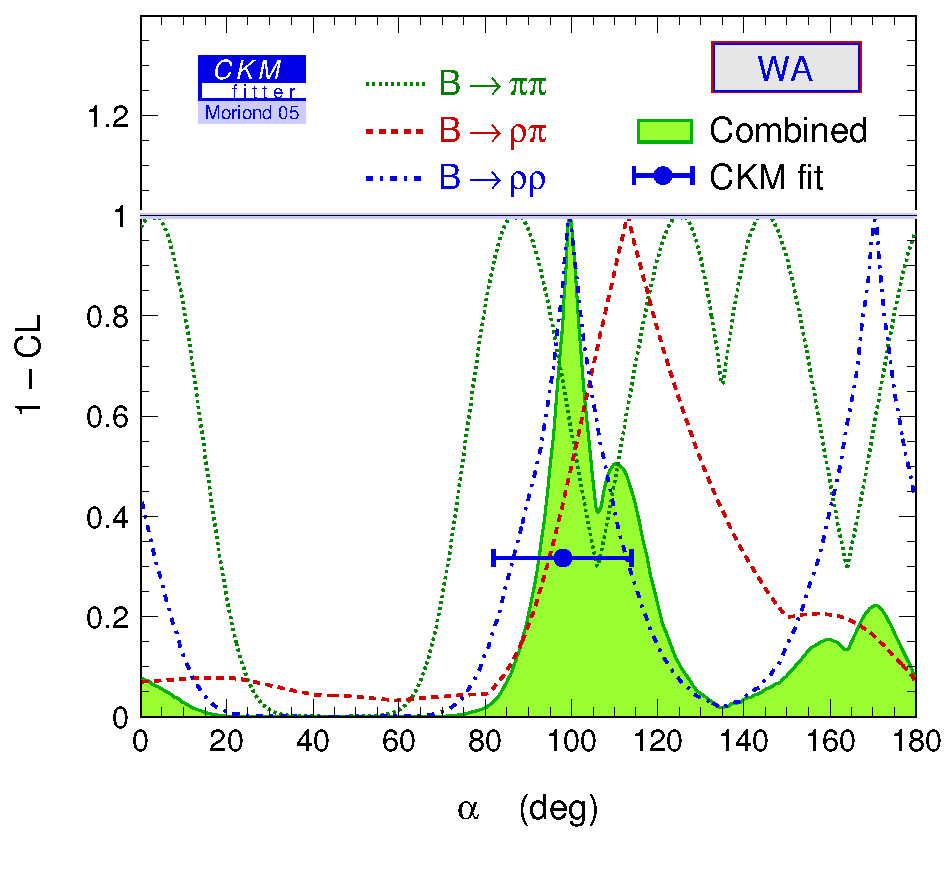
\includegraphics[width=\largefigwidth]{ckmfitter-alpha-combined}
  \caption{CKM Fitter constraints on \alphaCKM.}
  \label{fig:CKMFitter}
\end{figure}
\end{fsnippet}

Note also that this way of including images will automatically look for an
|.eps| file when building PostScript and a |.pdf| file when building PDF. You
may find the |eps2pdf| and |pdf2eps| utilities useful.

\subsection{Standard in-document reference terms}
It's nice to be able to refer to portions of your document with standard names,
capitalisation, etc. For this reason, I've defined a bunch of macros which give
consistent and sensible capitalisations. Using them systematically will ensure
consistency in your references:
%
\begin{itemize}
\item \texcmd{Chapter} \manifestsAs Chapter
\item \texcmd{Section} \manifestsAs Section
\item \texcmd{Appendix} \manifestsAs Appendix
\item \texcmd{Figure} \manifestsAs Figure
\item \texcmd{Table} \manifestsAs Table
\item \texcmd{Equation} \manifestsAs equation
\item \texcmd{Reference} \manifestsAs reference
\item \texcmd{Page} \manifestsAs page
\end{itemize}

Taking this consistency thing a step further, here are versions of the same
commands which take the reference label as a argument:
%
\begin{itemize}
\item \texcmd{ChapterRef}
\item \texcmd{SectionRef}
\item \texcmd{AppendixRef}
\item \texcmd{FigureRef}
\item \texcmd{TableRef}
\item \texcmd{EquationRef}
\item \texcmd{ReferenceRef}
\item \texcmd{PageRef}
\end{itemize}
%
Using these forms will ensure that the spacing between e.g. the worked
``Chapter'' and the chapter number is always the same, and that it won't wrap
over line breaks. The equation, reference and page forms will call the
\texcmd{eqref}, \texcmd{cite} and \texcmd{pageref} reference macros rather than
\texcmd{ref}, which is used for all others.

% \subsection{``thesis---'' prefix versions}
% Additionally, all \hepthesis environments and commands have an alternative name,
% which is the version described above, prefixed with ``thesis''\footnote{This
%   is a hang-over from early versions of my thesis, when I didn't know how to
%   robustly extend and re-define environments and commands.}. These forms are
% frankly a bit of a pain to use, so use the short versions, please. The
% ``thesis---'' versions should be considered deprecated and \textbf{will be removed
% in the next release, version 1.5}.


\section{Recommended extra packages}
\label{sec:ExtraPackages}
Here are some other packages it might be good to know about:
\begin{itemize}
\item \textbf{SIunits\,\cite{SIunits}:} \emph{the} way to do units and get it right.
\item \textbf{hepunits\,\cite{hepunits}:} my extension of |SIunits| to include some common HEP units not used elsewhere.
\item \textbf{hepnames\,\cite{hepnames} and hepparticles\,\cite{hepparticles}:} my packages for typesetting HEP particle names \emph{properly}, with |hepnames| defining macros for a lot of the standard ones. Requires |maybemath|\,\cite{maybemath}
\item \textbf{braket\,\cite{braket}:} decent implementation of Dirac bra and ket notation
\item \textbf{cancel\,\cite{cancel}:} the best way to do Feynman slashes (in my opinion)
\item \textbf{feynmf/feynmp\,\cite{feynmf} and axodraw\,\cite{axodraw}:} various approaches to doing Feynman diagrams, especially in equations, inline contexts and so-on.
\end{itemize}
%
and some related software:
%
\begin{itemize}
\item \textbf{FeynDiagram\,\cite{feyndiagram} and Jaxodraw\,\cite{jaxodraw}}: for Feynman diagrams outside \TeX. You might also
  be interested in my |pyfeyn|\,\cite{pyfeyn} program.
\item \textbf{SLAC SPIRES' biblio tools service:} see \url{www.slac.stanford.edu/spires/}
\end{itemize}



\section{An example \texttt{hepthesis} thesis}
Here are some selected snippets from my thesis, which hopefully demonstrate the
features described. I split my thesis into |preamble.tex| and
|thesis.tex| files, with the front matter, back matter and chapters
\texcmd{input}'d into |thesis.tex|. The output was built by running e.g.
%
\begin{snippet}
pdflatex thesis.tex && bibtex thesis && pdflatex thesis.tex
\end{snippet}
%
(though I used a Makefile rather than do it directly). You should note that you
might not be able to build this exact thesis due to missing packages: if you're
writing a HEP thesis then I'd encourage you to use the |hepnames| \LaTeX{}
package for typesetting particle names --- it depends on the extra
|hepparticles| and |maybemath| packages. The
examples used here also rely on the |hepunits| package: you can all these extra
packages from the CTAN\,\cite{CTAN}. See Appendix~\ref{app:InstallingPackages} for
a quick guide on how to install personal copies of \LaTeX{} packages.


\subsection{\texttt{preamble.tex}}
{\smaller \VerbatimInput{example/preamble.tex}}

\subsection{\texttt{thesis.tex}}
{\smaller \VerbatimInput{example/example.tex}}

\subsection{\texttt{frontmatter.tex}}
{\smaller \VerbatimInput{example/frontmatter.tex}}

\subsection{\texttt{chap1.tex}}
{\smaller \VerbatimInput{example/chap1.tex}}

\subsection{\texttt{chap2.tex}}
{\smaller \VerbatimInput{example/chap2.tex}}

\subsection{\texttt{backmatter.tex}}
{\smaller \VerbatimInput{example/backmatter.tex}}


\section{Wishlist / TODO}
I'm not planning on writing another thesis, but maybe I'll add features if
there's demand. If you add a nice feature, pass it on to me and I'll think about
including it in the package (and will give you some credit, of course). But anyway,
here's the TODO:
%
\begin{itemize}
\item Make the spacing in the \texcmd{SectionRef} etc. commands customisable.
\item Allow the PDF page style to be specified as a class argument
\item Allow section titles to be centre / right justified?
\item User control of frontmatter title sizes and alignments? (Probably not\dots)
\item Provide different styles for the titlepage etc.
\item Themes, like for Beamer?
\item Make the vertical spacings on the quote, dedication and title pages change by paper size
\end{itemize}


\section{Feedback}
\hepthesis has taken a lot of work\dots I hope you think it was worthwhile and
that you enjoy using it. Or at least, I hope you enjoy writing your thesis more
than you would have done without it! If you're feeling appreciative, then a teeny
credit in your thesis acknowledgements would be hugely appreciated.

Other than that, any feedback on the package is very welcome, especially if it's
constructive criticism! Email your thoughts to
\texttt{hepthesis@insectnation.org}, please.


\section{Acknowledgements}
I'd like to thank all the people who have provided bug reports, patches, suggestions
and who have otherwise helped me to get \hepthesis to the state it's in. See the
|ChangeLog| file in the distribution for names!


\appendix

\section{Using your own derived document class}
\label{app:DerivedClass}
If you're feeling sophisticated, then you can make your own document class based on
\hepthesis by placing
%
\begin{snippet}
\LoadClass{hepthesis}
\end{snippet}
%
in your own class definition file. This is a rather nice way of working, since
it allows you to tweak the \hepthesis defaults without cluttering your
|.tex| file with preamble junk.


\section{Installing personal copies of \LaTeX{} packages}
\label{app:InstallingPackages}
Since |hepthesis| depends on several non-standard \LaTeX{} packages, you may have to
download and install them yourself. If you don't have |root| access to the computer
on which you're working then you'll probably have to install them into your own home
directory or similar. Since I expect quite a few prospective users of |hepthesis| will
be non-experts in the ways of \TeX{}, this is a quick guide on what to do.

\begin{enumerate}
\item Make a \TeX{} directory tree in your home directory (or any other area you can write to), e.g.
\begin{snippet}
$ mkdir -p $HOME/local/texmf/tex/latex
$ mkdir -p $HOME/local/texmf/bibtex/bib
$ mkdir -p $HOME/local/texmf/bibtex/bst
\end{snippet}
\item Download the packages from CTAN\,\cite{CTAN} or wherever.
\item Follow the packages' installation instructions to install them into the \\
  |$HOME/local/texmf/tex/latex| %$
  directory you made above (or an appropriately-named sub-directory of it if you
  want to be neat). For simple |.sty| or |.cls| files, this will just involve
  copying them into your directory of choice. |.dtx| files will probably require
  running |latex| to build the files to be installed.
\item If you use the |bash| shell, add the following to your |~/.bashrc| file:
\begin{snippet}
export TEXINPUTS="$HOME/local/texmf/tex//:$TEXINPUTS"
export LATEXINPUTS="$HOME/local/texmf/tex/latex//:$LATEXINPUTS"
export BIBINPUTS="$HOME/local/texmf/bibtex//:$BIBINPUTS"
\end{snippet}
or, if you use the |(t)csh| shell, add the following to your |~/.cshrc| file:
\begin{snippet}
setenv TEXINPUTS "$HOME/local/texmf/tex//:$TEXINPUTS"
setenv LATEXINPUTS "$HOME/local/texmf/tex/latex//:$LATEXINPUTS"
setenv BIBINPUTS "$HOME/local/texmf/bibtex//:$BIBINPUTS"
\end{snippet}
\item That's all: the lines above mean that  \LaTeX{} will look for input files
such as classes, packages, images, \texcmd{input}'d |.tex| files etc. recursively under \\
|$HOME/local/texmf/tex/latex| %$
 and that BibTeX will look for its style and database files recursively under
|$HOME/local/texmf/bibtex|.%$
You can probably see how this can be extended to keep your thesis development
directories neat, too!
\end{enumerate}


\section{Distinguishing PS/PDF output in thesis builds}
\label{app:AuxFileProblem}

The options \texopt{bindnopdf} and \texopt{hyperpdf} change the behaviour
depending on whether you're building PDF or PostScript output. This is fine if
you only ever do one, but if you want to switch rapidly between these output
formats then you'll have problems. This is because the |.aux| file, which
records the reference keys and suchlike changes depending on whether you're
making hyper-refs and if the changes of margins force sections on to different
pages.

A nice solution to this involves using a Makefile, which you probably want to be
doing anyway. You'll have to read up on the details of Makefiles (and possibly
GNU automake) elsewhere, but to save on Make-newbie angst, I'll tell you that
the indents in the following snippet \emph{must} be tabs, rather than spaces!
Here goes --- put the following into a file called |Makefile|, change the
|DOCNAME| variable to something which suits your project and run |make thesis| or |make thesispdf|:
\begin{fsnippet}
# For a main thesis LaTeX file called ``thesis.tex''
DOCNAME = thesis

thesis: $(TEXSOURCES) $(DOCNAME).bbl
    test -f $(DOCNAME).aux.ps && cp $(DOCNAME).aux.ps \
      $(DOCNAME).aux || true
    latex $(DOCNAME)
    cp $(DOCNAME).aux $(DOCNAME).aux.ps
    ./thesisstats.sh >> buildlog.dat

thesispdf: $(TEXSOURCES) $(DOCNAME).bbl
    test -f $(DOCNAME).aux.pdf && cp $(DOCNAME).aux.pdf \
      $(DOCNAME).aux || true
    pdflatex $(DOCNAME)
    cp $(DOCNAME).aux $(DOCNAME).aux.pdf
    ./thesisstats.sh >> buildlog.dat
\end{fsnippet}

Otherwise you can just delete the |.aux| file when you change between using
|latex| and |pdflatex|, but this will require more passes, since the
|.aux| file has to be replaced each time.

\begin{thebibliography}{99}
\bibitem{CTAN}{CTAN: \url{http://www.ctan.org}. \url{http://www.tex.ac.uk/tex-archive} is shortened to |ctan:| below.}
\bibitem{scrbook}{scrbook: \url{ctan:/macros/latex/contrib/komascript/}}
\bibitem{cite}{cite: \url{ctan:/macros/latex/contrib/cite/}}
\bibitem{setspace}{setspace: \url{ctan:/macros/latex/setspace/}}
\bibitem{fancyhdr}{fancyhdr: \url{ctan:/macros/latex/contrib/fancyhdr/}}
\bibitem{rotating}{rotating: \url{ctan:/macros/latex/contrib/rotating/}}
\bibitem{tocbibind}{tocbibind: \url{ctan:/macros/latex/contrib/tocbibind/}}
\bibitem{subfig}{subfig: \url{ctan:/obsolete/macros/latex/contrib/subfig/}}
\bibitem{caption}{caption: \url{ctan:/macros/latex/contrib/caption/}}
\bibitem{ccaption}{ccaption: \url{ctan:/macros/latex/contrib/ccaption/}}
\bibitem{changepage}{changepage: \url{ctan:/macros/latex/contrib/changepage/}}
\bibitem{varwidth}{varwidth: \url{ctan:/macros/latex/contrib/varwidth/}}
\bibitem{csquotes}{csquotes: \url{ctan:/macros/latex/contrib/csquotes/}}
\bibitem{babel}{babel: \url{ctan:/macros/latex/contrib/babel/}}
\bibitem{a4wide}{a4wide: \url{ctan:/macros/latex/contrib/misc/a4wide.sty}}
\bibitem{amsmath}{amsmath: \url{ctan:/macros/latex/required/amslatex/math/}}
\bibitem{hyperref}{hyperref: \url{ctan:/macros/latex/contrib/hyperref/}}
\bibitem{booktabs}{booktabs: \url{ctan:/macros/latex/contrib/booktabs/}}
\bibitem{draftcopy}{draftcopy: \url{ctan:/macros/latex/contrib/draftcopy/}}
\bibitem{lineno}{lineno: \url{ctan:/macros/latex/contrib/lineno/}}
\bibitem{titling}{titling: \url{ctan:/macros/latex/contrib/titling/}}
\bibitem{SIunits}{SIunits: \url{ctan:/macros/latex/contrib/SIunits/}}
\bibitem{hepunits}{hepunits: \url{ctan:/macros/latex/contrib/hepunits/}}
\bibitem{hepnames}{hepnames: \url{ctan:/macros/latex/contrib/hepnames/}}
\bibitem{hepparticles}{hepparticles: \url{ctan:/macros/latex/contrib/hepparticles/}}
\bibitem{maybemath}{maybemath: \url{ctan:/macros/latex/contrib/maybemath/}}
\bibitem{braket}{braket: \url{ctan:/macros/latex/contrib/misc/braket.sty}}
\bibitem{cancel}{cancel: \url{ctan:/macros/latex/contrib/misc/cancel.sty}}
\bibitem{feynmf}{feynmf: \url{ctan:/macros/latex/contrib/feynmf/}}
\bibitem{axodraw}{axodraw: \url{http://www.nikhef.nl/~form/FORMdistribution/axodraw/}}
\bibitem{feyndiagram}{FeynDiagram: \url{http://www.feyndiagram.com}}
\bibitem{jaxodraw}{Jaxodraw: \url{http://http://jaxodraw.sourceforge.net/}}
\bibitem{pyfeyn}{PyFeyn: \url{http://hepforge.cedar.ac.uk/pyfeyn/}}
\end{thebibliography}

\end{document}
